\section{Task and Data}

\paragraph{Outputs and legal states.}
The task predicts four fields for each paragraph. We study the AI CUP
VeriPromise\hspace{0pt}ESG development release.
Promise status (PS) is \emph{Yes} or \emph{No}. Verification timeline (VT) is
\emph{already}, \emph{within two years}, \emph{between two and five years},
\emph{more than five years}, or \emph{N/A}. Evidence status (ES) is
\emph{Yes}, \emph{No}, or \emph{N/A}; evidence quality (EQ) is \emph{Clear},
\emph{Not Clear}, \emph{Misleading}, or \emph{N/A}. These fields obey hard
implications: PS=No requires VT=ES=EQ=N/A, whereas PS=Yes requires one of the
four substantive timelines and ES in \{Yes, No\}. In turn, ES=No requires
EQ=N/A, whereas ES=Yes requires one of the three substantive quality labels.
Thus the Cartesian label space has $2\times5\times3\times4=120$
combinations, but only
\begin{equation}
  1+4(1+3)=17
  \label{eq:legal-states}
\end{equation}
legal tuples: one for PS=No, and for each of four timelines either one ES=No
state or three ES=Yes quality states.

\begin{figure*}[t]
  \centering
  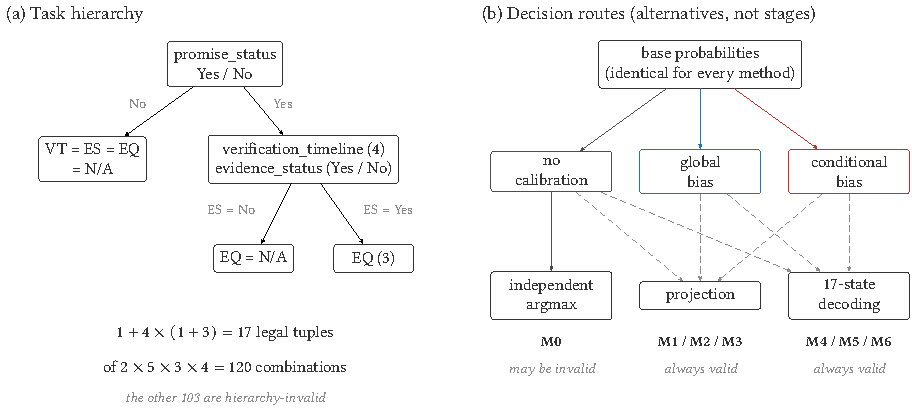
\includegraphics{../figures/figure1_hierarchy.pdf}
  \caption{The task hierarchy and the alternative decision routes. All routes
  consume identical base probabilities; projection and 17-state decoding
  guarantee a legal tuple, whereas independent argmax does not.}
  \label{fig:hierarchy}
\end{figure*}

\paragraph{Development-set audit.}
The release contains 2,000 labeled development paragraphs from 49 source
reports covering 50 companies, and it realizes 15 of the 17 legal states
(Table~\ref{tab:dataset}). The rarest EQ label,
\emph{Misleading}, has only two instances; we therefore make no improvement
or significance claim for that class.

\begin{table}[t]
  \centering
  \caption{Dataset summary from the frozen study artifact.}
  \label{tab:dataset}
  \begin{tabular}{lrr}
\toprule
Statistic & Development & Competition test \\
\midrule
Paragraphs & 2000 & 2000 \\
Source reports (PDFs) & 49 & 49 \\
\quad shared with other split & 49 & 49 \\
Companies & 49 & 49 \\
Gold labels available & Yes & No \\
Gold hierarchy-valid tuples & 2000 / 2000 & n/a \\
Legal states observed & 15 / 17 & n/a \\
\midrule
\multicolumn{3}{l}{\emph{Rarest classes}} \\
\quad within\_2\_years & 34 & n/a \\
\quad Misleading & 2 & n/a \\
\bottomrule
\end{tabular}

\end{table}

All 49 development reports also occur in the unlabeled competition test data,
and one paragraph text occurs in both splits. This overlap describes sources
and text only: because competition test labels are unavailable, we infer no
label-derived test statistic. No company contributes more than one report;
one report covers two companies. Consequently, in this corpus a
document-disjoint split is necessarily company-disjoint, rather than a
separate company-level experiment.
